\section{Experiments}
\label{sec:experiment}


In the following section, we give a description of our datasets and outline the structure of our experiments, which include two separate prediction tasks. We also define important measures that will be used to assess competing methods. Finally, we present results from our experiments and evaluate the effectiveness of each method.

\subsection{Data Sets}  \label{data:sets}
\scriptsize
\begin{center}
\begin{table}[h!]
\begin{tabular}{|c|c|c|c|c|c|c|c|c|c|c|c|c|c|} 
 \hline
  & Asian Pct. & Black Pct. & Hispanic Pct. & White Pct. & Income Ent. & Population Ent. \\
 \hline
 2010 & 0.05 & 0.41 & .21 & .34 & 1.29 &  0.64 \\
 \hline
\end{tabular}
\caption{Urban data summary statistics. All figures are averaged over community areas. We report the average population percentage by race/ethnicity. Additionally, we compute the average entropy of income and and population over race. These measure of entropy indicate how much income and population differ by race.}
\label{summaryStatsX}
\end{table}
\end{center}

\normalsize


\textbf{Demographics Data} We study urban dynamics as in \cite{wang:region}. The data set contains a set of features describing geographic sub-regions in the metropolitan area of Chicago, IL. The fundamental geographic unit of analysis is called a tract, and is provided by the US census survey \cite{census:2010}.

Additionally, we collect a set of tract-level demographic data also published by the U.S. Census Bureau \cite{census:2010}. For instance, we observe income distribution by race and ethnicity in each census tract. We utilize these, and other features, in our predictive model, (equation \ref{regression:mod}), by first aggregating to the proposed community level, $\mathcal{Z}'$, using an aggregation function, $g$. This demographics data set provides estimates of total population, population density, poverty, residential stability, and ethnic diversity.


\begin{center}
\begin{table}[h!]
\begin{tabular}{|c|c|c|} 
 \hline
  & Crime Count & House Price \\
 \hline
 2010 & 4787.04 & 168.52  \\
  \hline
 2011 & 4556.61 & 179.45  \\
 \hline
\end{tabular}
\caption{Summary statistics of the target variables by year. We report the mean crime count and house price (per square foot) for both our 2010 (training) and 2011 (test) data sets.}
\label{summaryStatsY}
\end{table}
\end{center}

To demonstrate that our proposed method is effective over multiple tasks, we perform two experiments. In both empirical studies, we rely on a common set of features, but change the prediction task of the learning algorithm. We briefly describe the tasks here, and give a full summary and discussion of results in section \ref{results}. 

\textbf{Crime Data}. We begin by studying crime counts in Chicago. Data related to Chicago-area crime is collected from the Chicago Data Portal~\cite{data-crime}, which is comprised of records of over five million incidents of crime from 2011 - 2017. Our study focuses on 2010 and 2011 only. In this publicly available data set, we observe the date, location and type of each crime incident. Our goal is to then learn a function that can predict the number of crimes in a given community-area, conditional on a proposed partition, $\mathcal{Z}'$. When evaluating the test error of our model, we first temporally split our training data. Meaning, we hold out data from 2011 as the test data and train the model on data from 2010. Table \ref{summaryStatsY} provides summary statistics for the response variable, $Y_i$, by year.

\textbf{House Price Data}. Next, we obtain house price estimates of real estate properties in the Chicago metropolitan area~\cite{data-houseprice}. We observe price, floor size, and latitude and longitude information for over 45,000 properties that sold within a two-year period. Our goal in this task is to then predict sale price per square foot conditional on our proposed partition, $\mathcal{Z}'$. Again, we rely on the same temporal test-train splitting strategy for evaluation.

\subsection{Experimental Settings}
\subsubsection{Benchmarks}\label{benchmarks}
In section \ref{sec:method} we introduced three methods that automatically learn both parameters, of interest: $\mathcal{Z}$, the discrete, region partition structure, and $\theta$, the parameters of a predictive model. To the best of our knowledge, these three methods, which we refer to as Naive MCMC, Guided MCMC, and Q-learning, are new to the domain of learning geo-spatial partitions. We compare these proposed methods to various benchmarks.  

The first benchmark is simply the given administrative boundary, as defined by the U.S. Census Bureau. Rather than learn an optimal partition, $\mathcal{Z}^*$, we take the partition as given, $\mathcal{Z}^0$, and learn a function to predict $Y_i$. A visual depiction of the partition, $\mathcal{Z}^0$, is found in figure \ref{fig:intro}.


The second benchmark is an agglomerative clustering algorithm, which is an unsupervised learning technique well-known to the literature \cite{hastie:book}. The agglomerative clustering algorithm is a bottom-up, hierarchical clustering method.  The algorithm begins with each tract in its own singleton cluster and recursively merges the pair of clusters that exhibits the smallest intergroup dissimilarity. If $\mathcal{G}$ and $\mathcal{H}$ represent two sets of tracts, or clusters, then we can define the dissimilarity between them as $d(\mathcal{G},\mathcal{H})$. A variety of choices exist for the selection of $d$, such as single linkage, complete linkage, and ward linkage. At each step, the two partitions with the smallest dissimilarity, $d$, are merged. This clustering technique is especially useful in the case of region partitioning because it allows for use of a connectivity matrix, which defines pairwise connections between data points, or tracts. This restricts the algorithm to only consider merging existing regions that are spatially connected.
\subsubsection{Measures} To holistically assess the quality of our proposed methods, we want to understand the behavior of each approach on two dimensions. 

First, we want to gain an understanding of the prediction accuracy of each model conditional on its optimal state, $\mathcal{Z}^*$. To measure accuracy, we compute the mean absolute error (MAE) using a leave-one-out (LOO) cross validation strategy. We use community area as the base unit in our LOO evaluation. Due to the stochastic nature of our methods, we perform a simulation study wherein we learn each model $n$ times.
For each model simulation iteration, $i = 1,...,n$, we compute the LOO MAE score. We then compute the mean and resulting standard deviation over iterations,$i = 1,...,n$, to obtain a single diagnostic measure for accuracy.

Next, we desire a measure that captures the stability of the model, or the degree to which different iterations of the same model produce the same optimal partition, $\mathcal{Z}^*$. To measure stability, we use the Adjusted Rand Index \cite{rand:hubert}, which measures the correspondence of two different partitions of a finite set of objects. The measure is attractive, because it accounts for agreement and disagreement of pairs of objects. Furthermore, the Adjusted Rand Index corrects for chance agreement between pairs using the generalized hyper-geometric distribution. The index achieves a value of 0 when two partitions were generated completely randomly, and value of 1 when the partitions are exactly equal \cite{rand:hubert, ml:murphy}. We compute the mean Adjusted Rand Index $n$ times for each algorithm in our simulation study. \\

%Lastly,  we hope to gauge how quickly and efficiently each proposed solution is able to find the optimal partition, $\mathcal{Z}^*$. The sequential nature of each proposed solution leads to the obvious metric of the number of iterations required until our convergence criterion, $\epsilon$, is reached. As part of our simulation study, we learn each model $n$ times and compute the mean number of iterations to convergence for each method. For consistency, we hold $\epsilon$ constant across all simulations. 
%


\subsection{Quantitative Evaluations} \label{results}

\subsubsection{Clustering Baseline}
We begin our quantitative evaluation by establishing empirical baselines using the two methods described in section \ref{benchmarks}. We estimate the regression model using both the administrative boundary, and the updated partition produced by the agglomerative clustering algorithm. To establish baselines of accuracy, we compute the MAE. Because both methods are inherently deterministic, they will arrive at the same result each time they are estimated. Therefore, in both cases the Adjusted Rand Index will always be 1. It is of little use of as diagnostic and we omit it below. Table \ref{baseline:table} contains results from both baseline methods. A visualization of the resulting partition from the agglomerative clustering algorithm is found in figure \ref{qlearn:fig}a.

It is obvious from table \ref{baseline:table} that the agglomerative clustering method gives very poor results, significantly increasing the MAE in both cases. Due to the poor performance of the agglomerative clustering algorithm, we will henceforth only use the administrative boundary as a baseline. 
\begin{center}
\begin{table}[h!]
\begin{tabular}{ |c|c|c| } 
\hline
  & MAE - crime  & MAE - house price\\
 \hline
 Admin. Boundary & 1715.91 & 31.29 \\ 
 \hline
 Agglomerative &72201.00 & 50.34 \\
 \hline
\end{tabular}
\caption{Evaluations of baseline methods on both crime and house price prediction. Admin. Boundary establishes the current state baseline. Obviously, the agglomerative clustering method performs poorly on both the crime and house price prediction tasks.}
\label{baseline:table}
\end{table}
\end{center}




\subsubsection{Description of Simulation Study}
Due to the stochastic nature of our proposed methods, we performed a simulation study and compared them on the basis of accuracy and stability. Specifically, using each method, $m$, we learn the  optimal partition, $\mathcal{Z}^*_{mi}$, for $i=1,...,n$. Setting $n=10$, we simulate and record the MAE. Additionally, we calculate the Adjusted Rand Index of all pairwise combinations of $\mathcal{Z}^*_{mi}$ to understand to what degree the method converges to the same solution. We perform this simulation for both crime and house price prediction. 



\subsubsection{Partition Effectiveness}\label{error:section}


\label{Crime} Results for the crime prediction task are found in table \ref{table:mae}. First, note that all three approaches in table \ref{table:mae} achieve a significant improvement over the baseline established using the administrative boundaries, which resulted in an error of 1715.91. This is much larger than that of the three proposed methods. Therefore, any one of the Naive MCMC, Guided MCMC, or Q-learning algorithms could be used to improve prediction error. Furthermore, can see that, on average, the Q-learning approach does indeed outperform both MCMC methods in terms of prediction error (MAE). We believe the Q-learning approach to be well-suited to the problem of identifying optimal community partitions. As a robustness check, we repeat the simulation study on a new task: average house price prediction. 

\begin{center}
\begin{table}[h!]
\begin{tabular}{ |c|c|c| } 
 \hline
  & MAE - crime & MAE - house price   \\
 \hline
 Admin. Boundary & 1715.9 & 31.29 \\
 \hline
 Naive MCMC & 1073.42 (81.93) & 25.73 (2.76)  \\ 
 \hline
 Guided MCMC & 1041.68 (76.75) & 27.13 (2.98)  \\ 
 \hline
 Q Learning & 746.13 (154.19) & 25.16 (1.30) \\  
 \hline
\end{tabular}
\caption{Mean absolute error for both the crime and house price prediction tasks}
\label{table:mae}
\end{table}
\end{center}

\label{HousePrice} Analysis of Table \ref{table:mae} for house price prediction results in conclusions that were similar to those in crime prediction task. First, all three methods of interest improve over the baseline administrative boundary. Second, the Q-learning algorithm is the method that minimizes test error. One interesting question arises regarding the relationship of the Naive and Guided MCMC methods. In the case of house price prediction, the Guided MCMC did not outperform the Naive MCMC like it did in the crime prediction task. Because the Guided MCMC relies on a proposal distribution with that is based on a biased heuristic, it is likely that it is not able to explore the full state space. This bias was especially apparent in the house price prediction task. For this reason, it is preferable to use the Q-Learning algorithm, which is able to learn the best sampling strategy from the data.

\begin{figure}[h]
\centering
%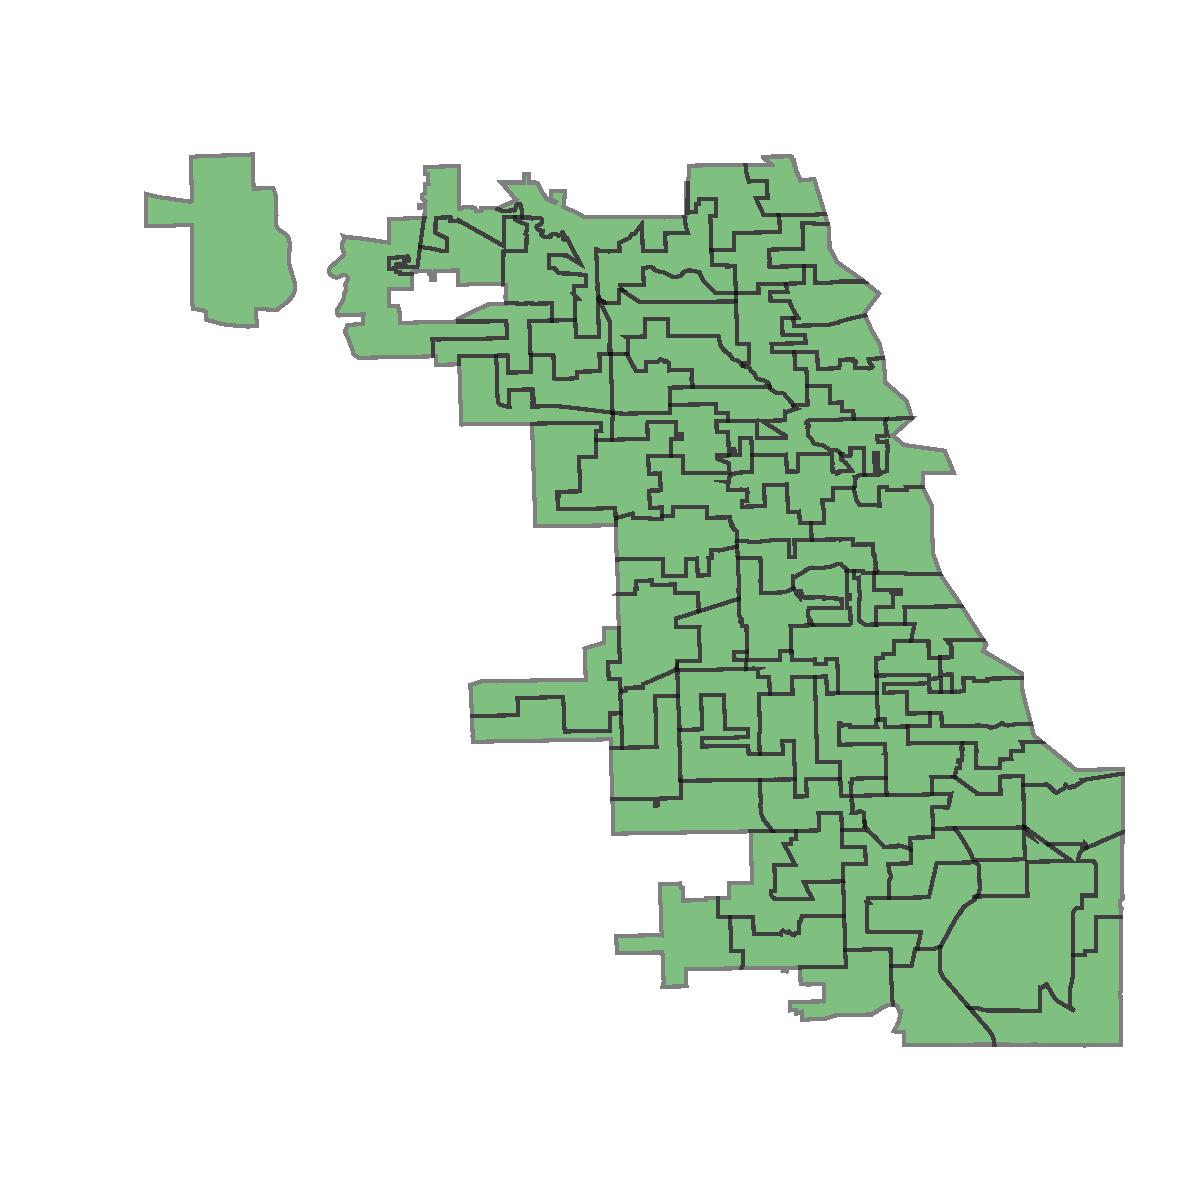
\includegraphics[width=0.5\linewidth]{fig/q-learning-v10-CAs.pdf}
\subfigure[Agglomerative]{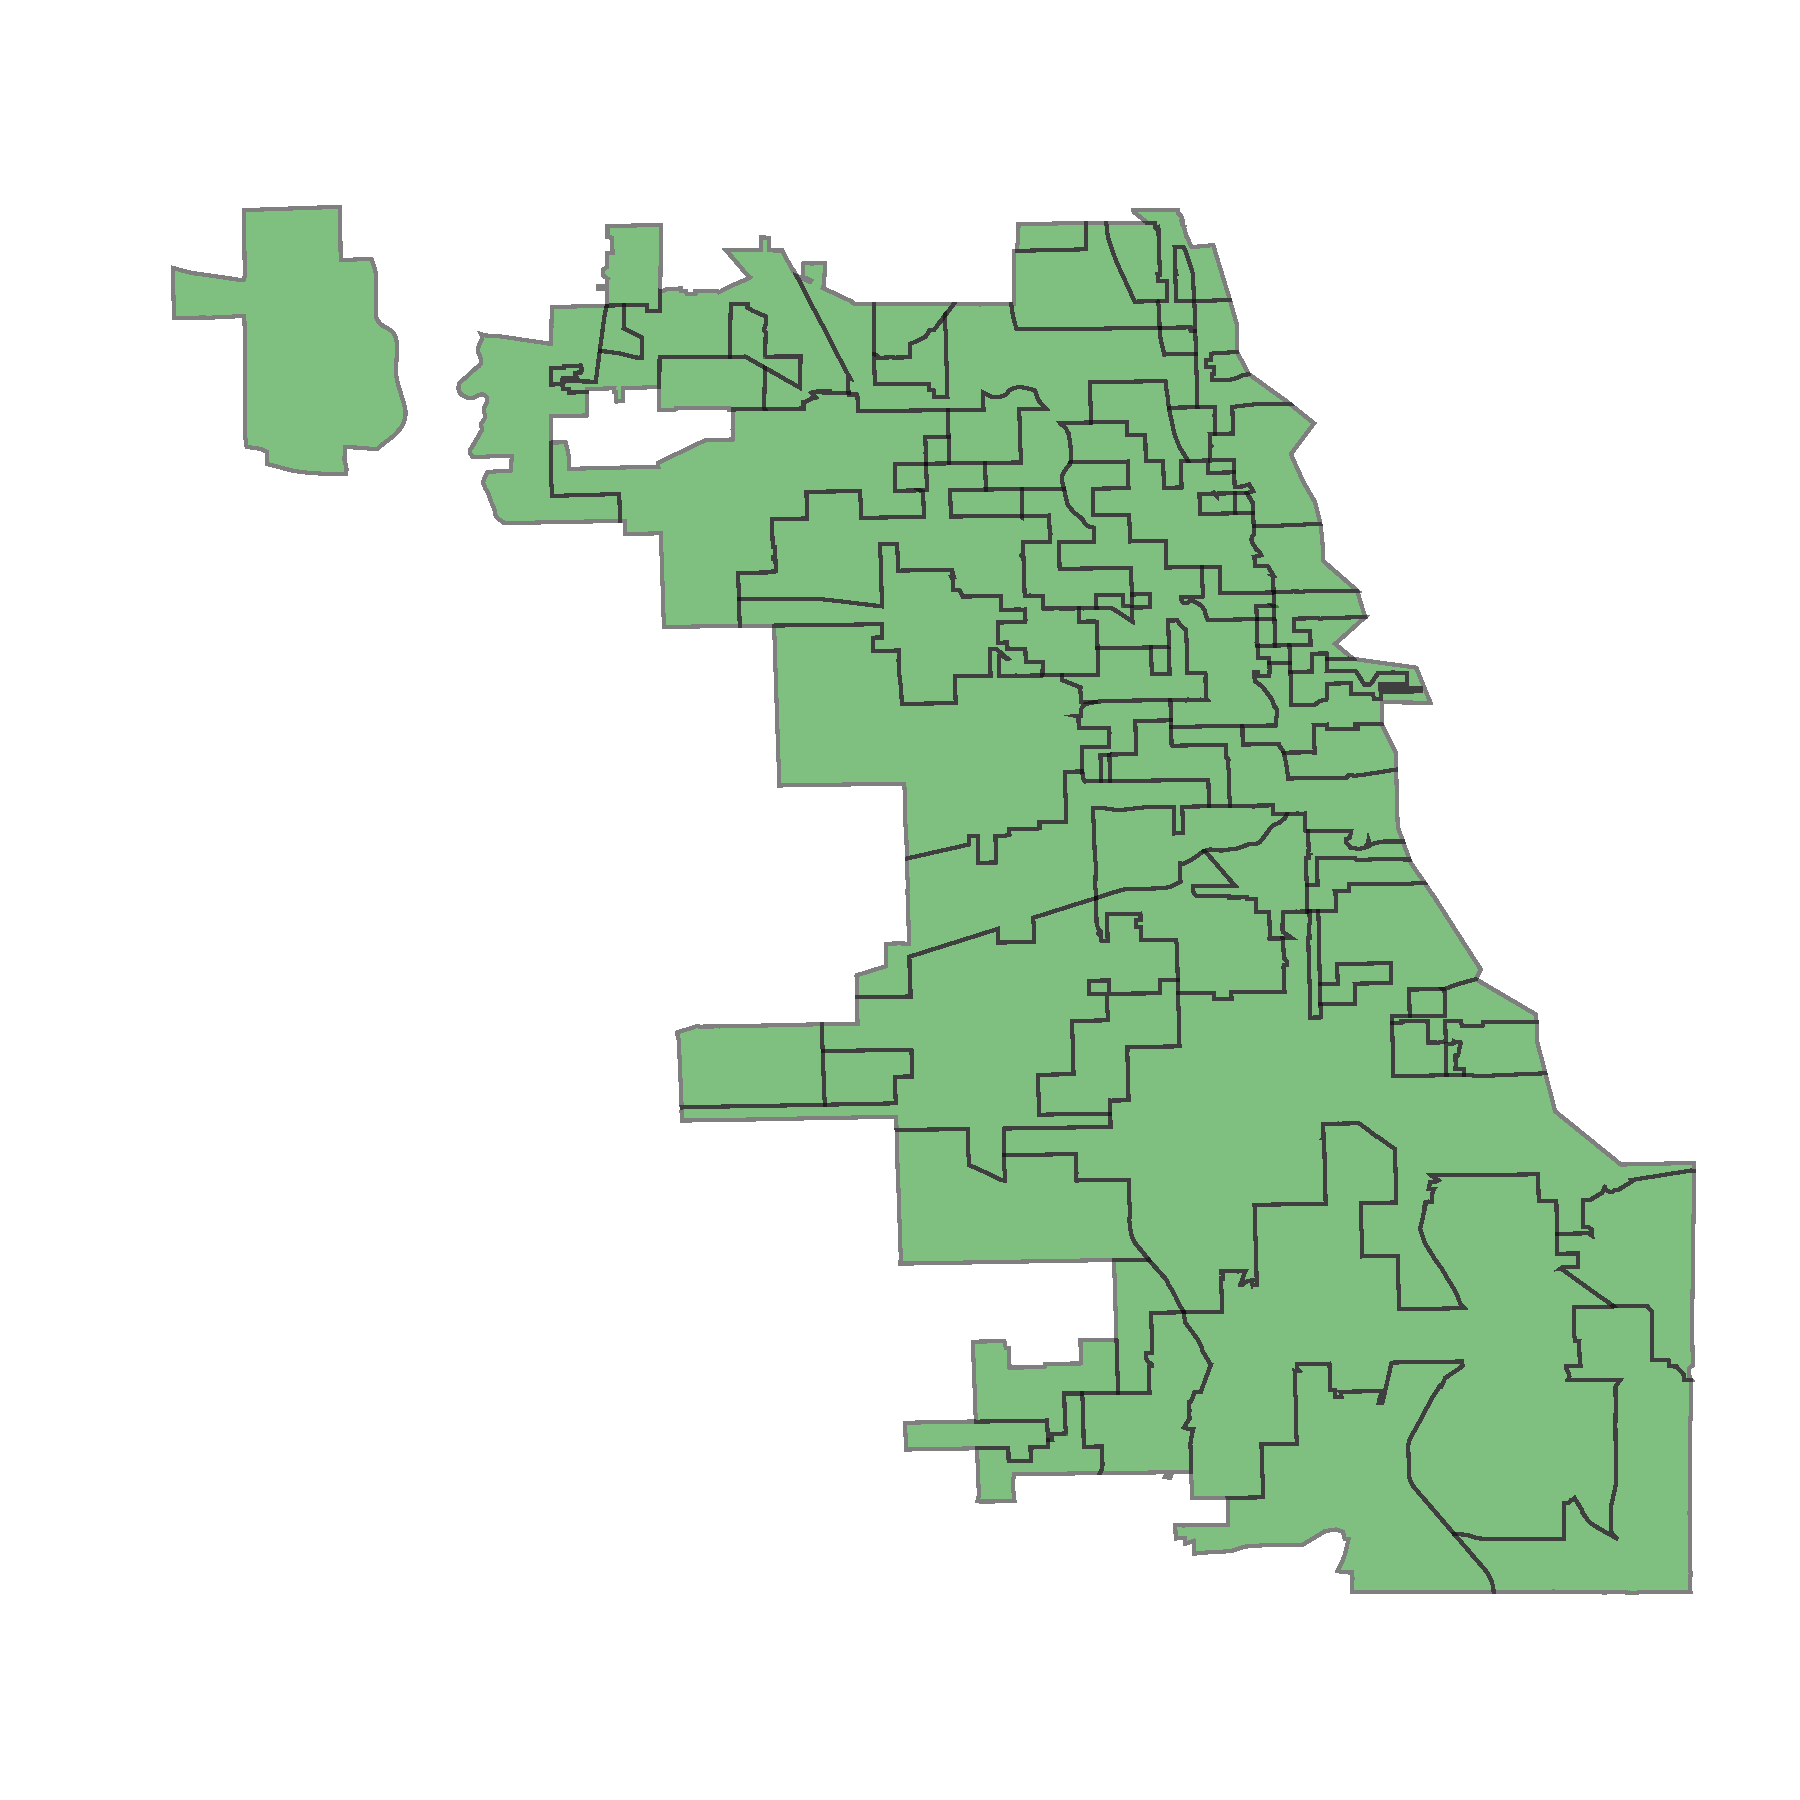
\includegraphics[width=0.45\linewidth]{fig/agg_CAs.pdf}}
\subfigure[Q-Learning]{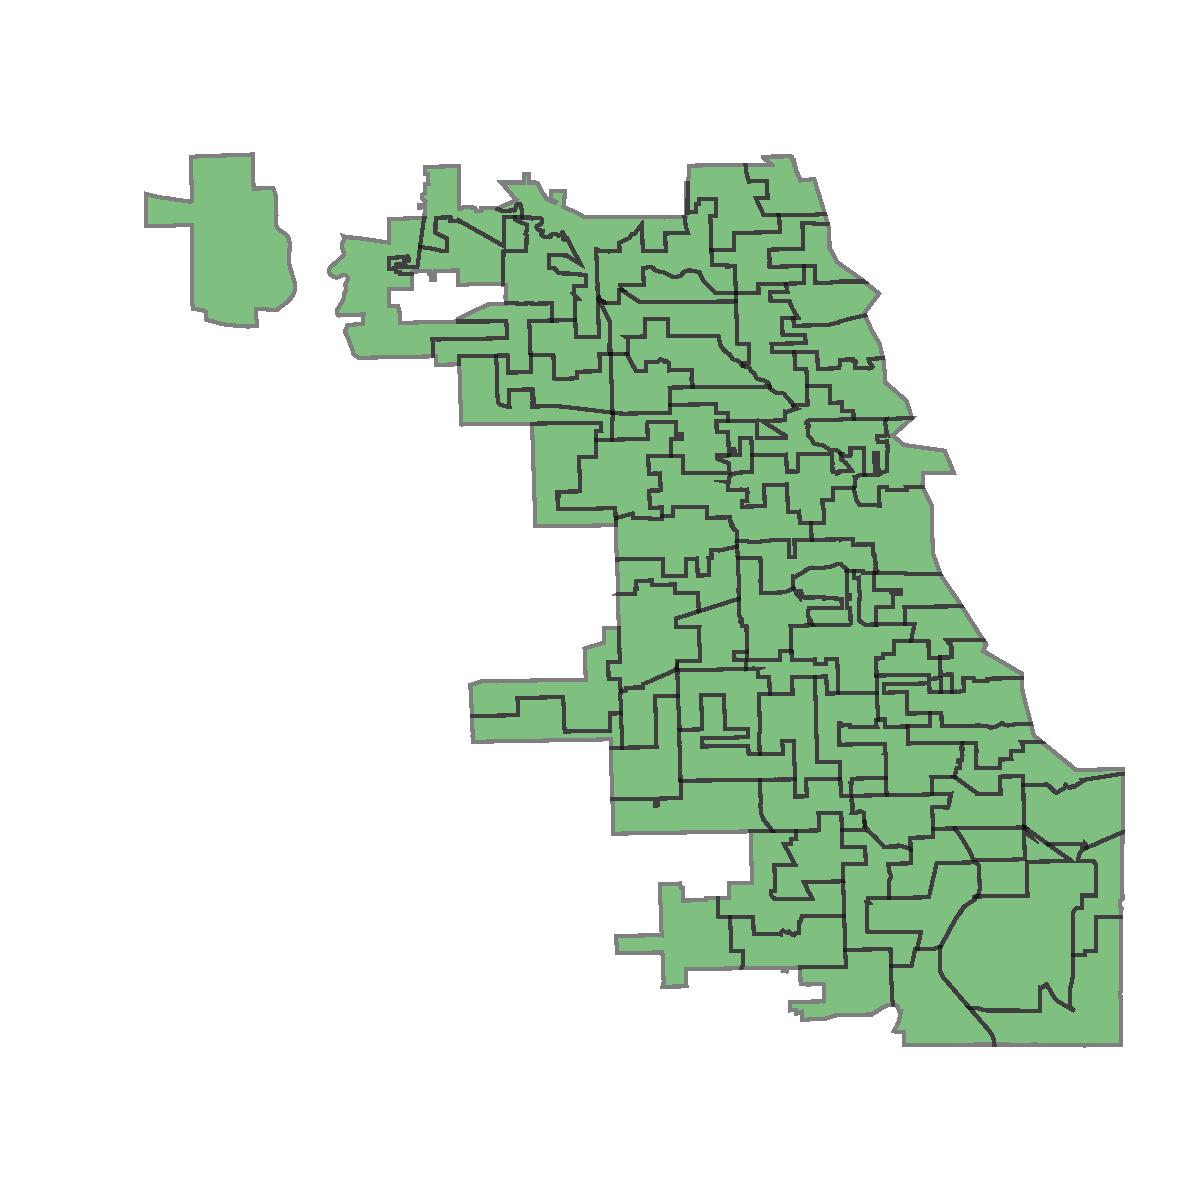
\includegraphics[width=0.45\linewidth]{fig/q-learning-v10-CAs.pdf}}

\caption{(a) Community partition from agglomerative clustering with ward linkage. The communities exhibit a large variance in geographic area, but more importantly, this partition yields large error for both prediction tasks. (b) Community partition from Q-learning}
\label{qlearn:fig}
\end{figure}

We conclude with a brief discussion of the convergence of our proposed method. One drawback of using MCMC in practice is the requirement of the user to assess whether the markov chain has truly converged to the target distribution. A very common technique, which we employ through the current work, is a simple visual analysis of trace plots to assess whether the chain converges \cite{ml:murphy}. Specifically, we impose a convergence criterion, $\epsilon$, on the objective function. We define $\epsilon$ as the standard deviation of the previous 100 values of the chain. If the standard deviation of these trailing values is less than 3, we end the algorithm. We then confirm with a visual diagnostic of the trace plot. In figure \ref{qlearn:convergence} we plot three quantities of interest as a function of iteration: MAE, the population variance of communities, and our objective function as defined in equation \ref{eq:boltzmann}. Recall that we constrain the optimization of the MAE with the population variance of communities, essentially preferring communities of equal size. We can see that this instance of the Q-learning algorithm converges in just over 350 iterations. 


\begin{figure}[h]
\centering
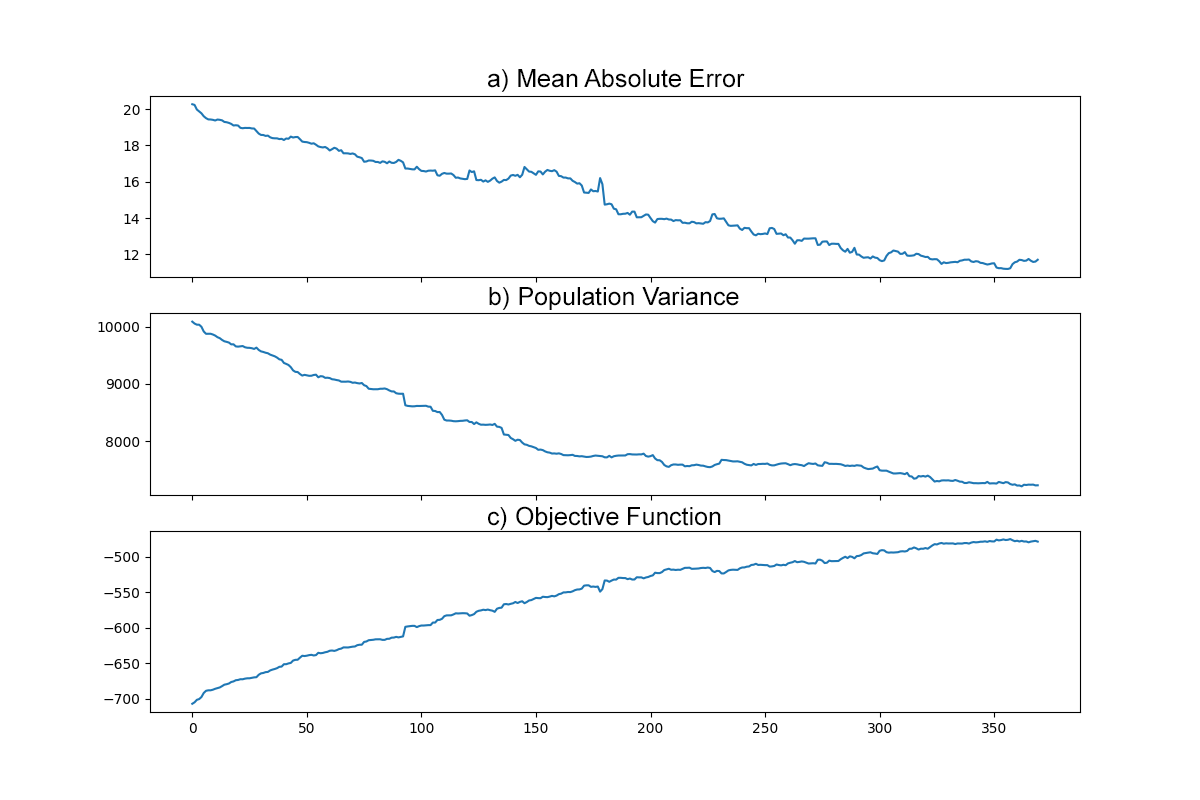
\includegraphics[width=1.0\linewidth]{fig/house-price-q-learning-sampler-v89.png}
\caption{Convergence plots from Q-learning}
\label{qlearn:convergence}
\end{figure}



\subsubsection{Partition Stability}
Previously, we analyzed the three methods in terms of accuracy relative to a baseline measure. Accuracy is arguably the most import basis of comparison, because it directly assesses our ultimate goal of prediction. However, we also are interested in comparing this methods in terms of stability. From table \ref{rand:table} we see a similar pattern over both tasks. In all cases, Naive MCMC is the least stable, Guided MCMC is the most stable, and Q-learning falls in between.  This is an interesting observation that guided MCMC, while not the most accurate method, is in fact the most stable. Our conclusion here is that the Guided MCMC is more consistently converging to slightly more similar partitions, but that these partitions are objectively worse than those from the Q-learning algorithm, as indicated by the errors measures in tables \ref{CrimeTable} and \ref{HousePriceTable}.
\begin{center}
\begin{table}[h!]
\begin{tabular}{ |c|c|c| } 
 \hline
    & Adj. Rand (Crime) & Adj. Rand (House Price) \\
 \hline

 Naive MCMC &  0.3645 (0.04) & 0.4982 (0.02) \\
 \hline
 Guided MCMC &  0.5550 (0.05) & 0.6702 (0.04)\\ 
 \hline
 Q-learning  &  0.4483 (0.03) & 0.6171 (0.03)\\  
 \hline
\end{tabular}
\caption{Adjusted Rand Index for the three proposed methods on each prediction task. We reported the mean and standard deviations of all pair-wise combinations of each method. The Ajdusted Rand Index measures the stability of each algorithm, or the degree to which different iterations converge to the same solution}
\label{rand:table}
\end{table}
\end{center}


%Conclusion:
%1. Q learning is more stable than Naive.
%2. Why Softmax mcmc cannot beat naive mcmc? Because the Softmax MCMC is biased to heuristics, and thus it cannot explore some search space.


\subsection{Case Study}
In section \ref{error:section} we show that the proposed Q-learning method identifies a community partition that significantly decreases prediction error over multiple tasks. However, one fair question one can raise about this method relates to the semantic meaning of the partitions the method chooses. In other words, how, or why, is the Q-learning algorithm arriving at the partition structure it does? To shed light on this question, we perform a qualitative, univariate study of the behavior of our model. Our goal here is only to help paint a more intuitive picture of one possible explanation of the partition selection process.
\begin{figure*}
\centering
\subfigure[All communities]{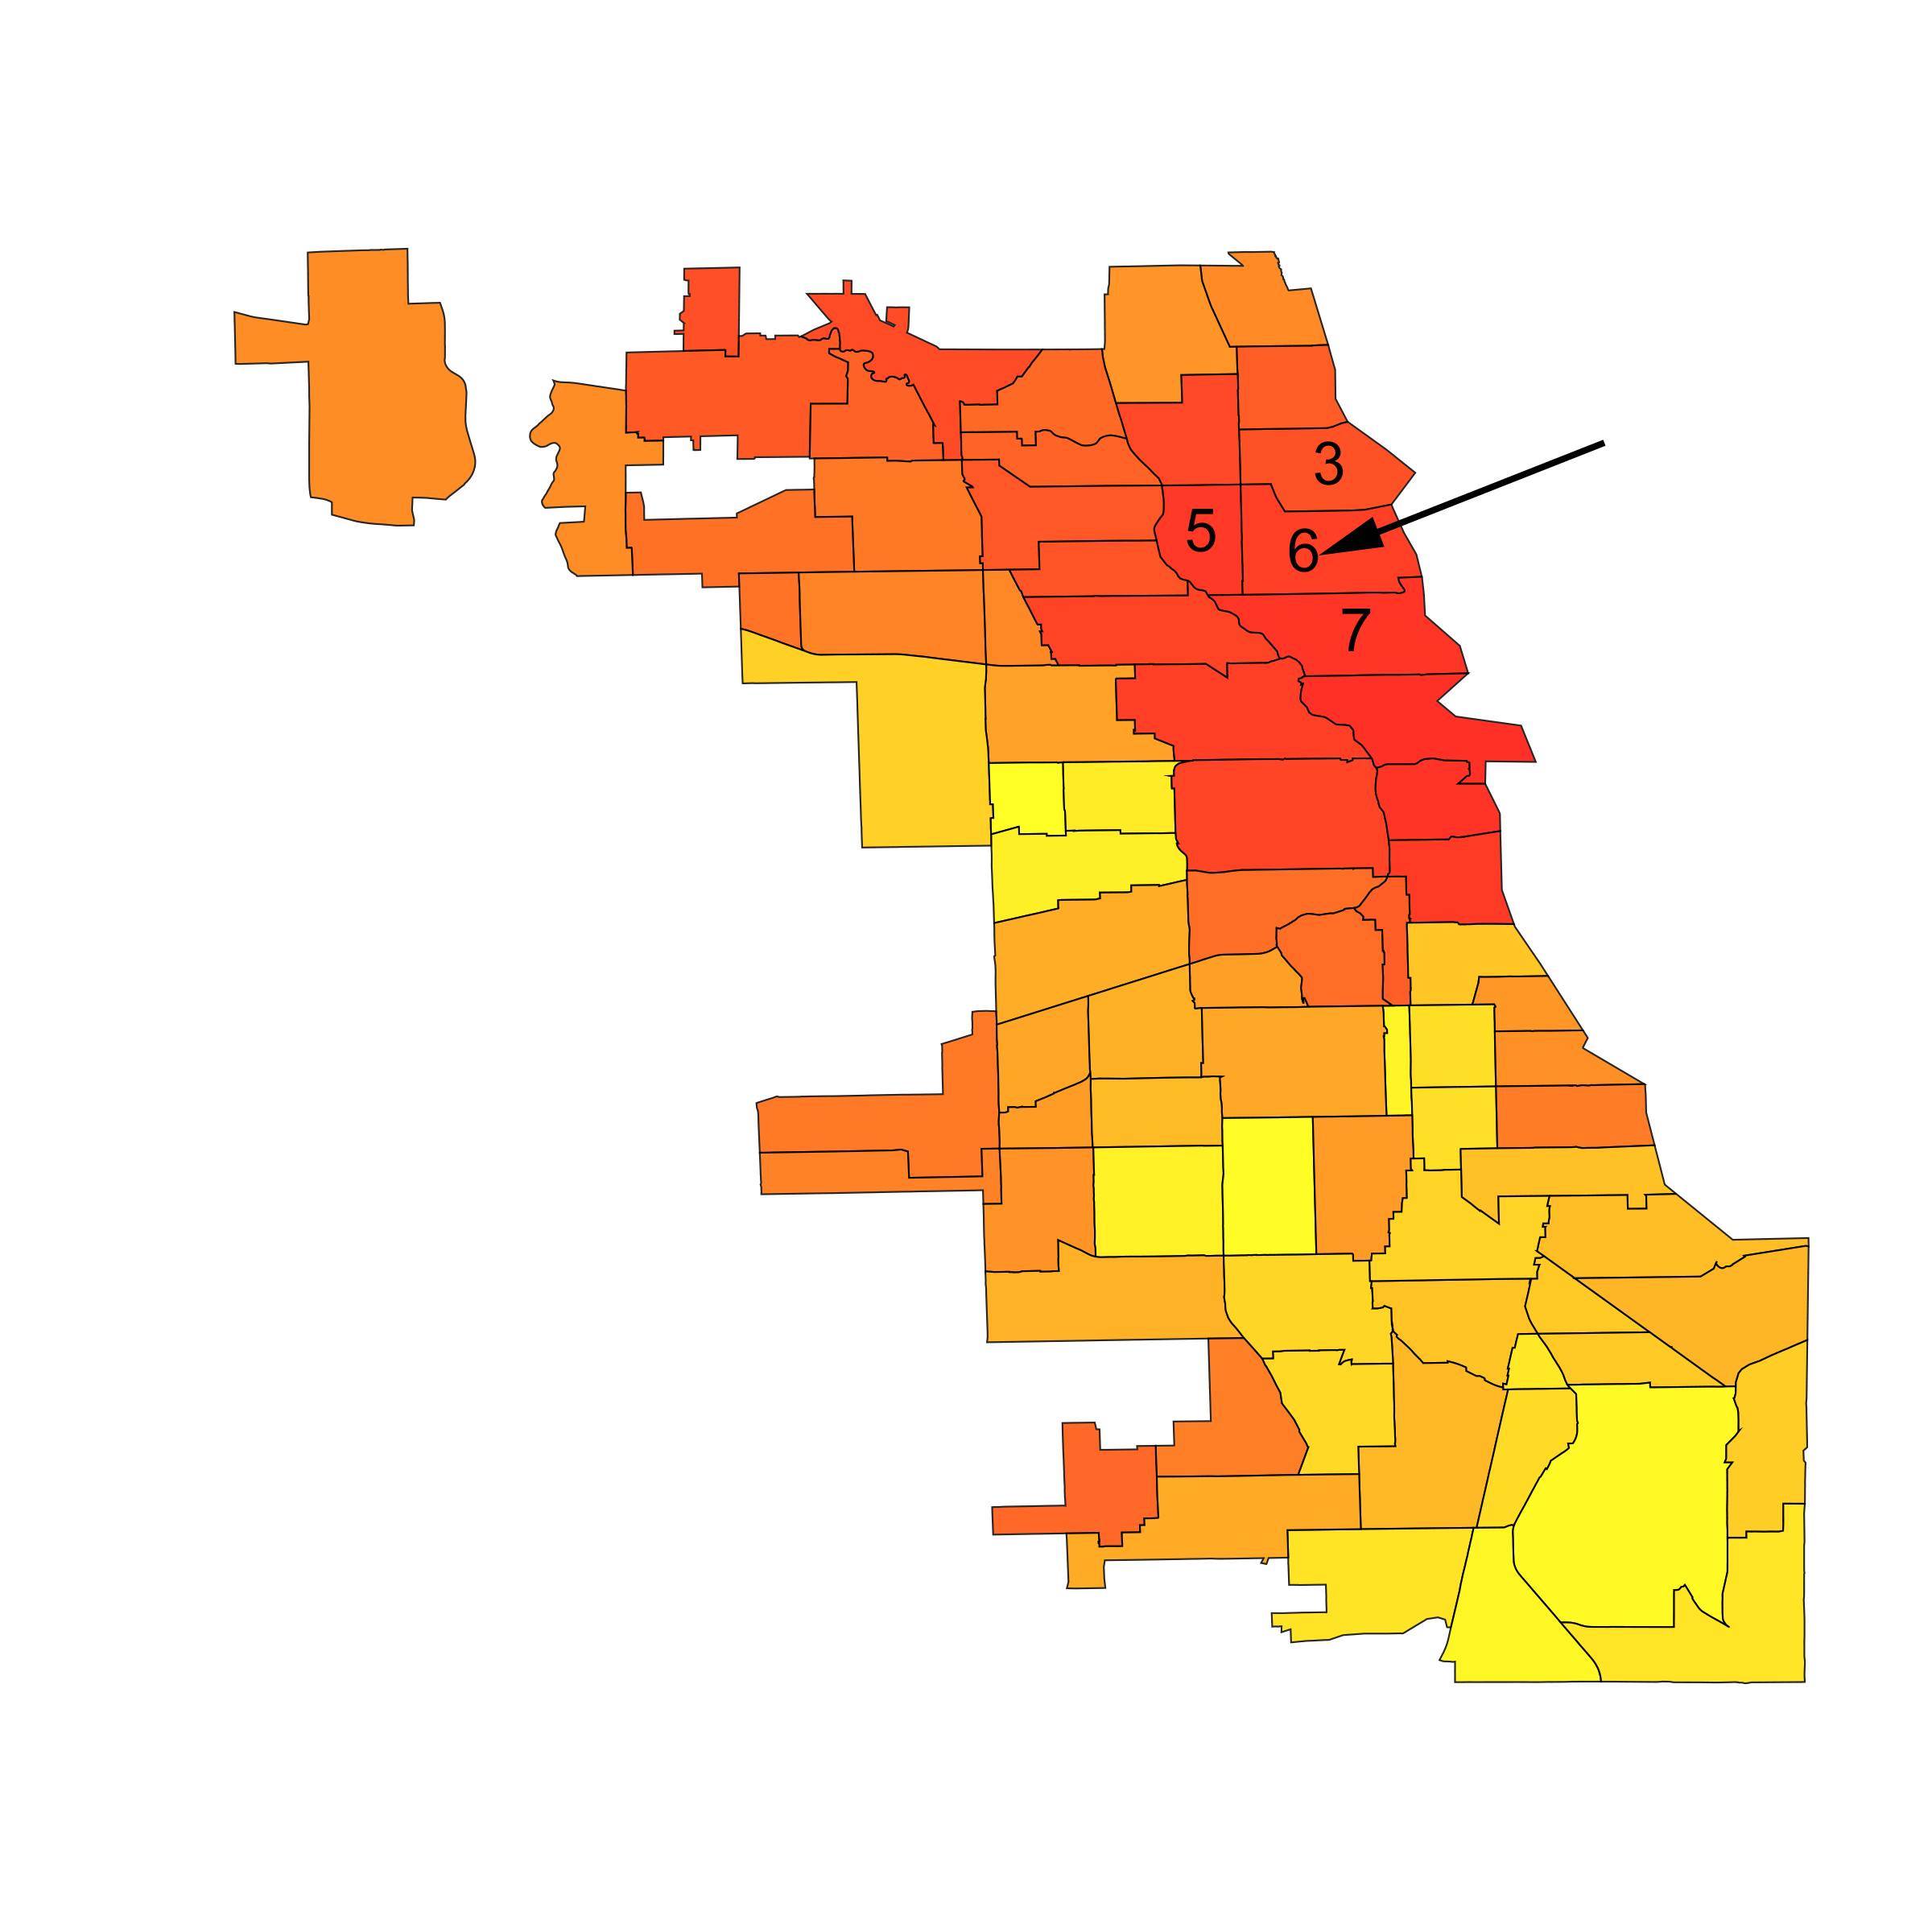
\includegraphics[width=0.2\linewidth]{fig/before-train_average_house_price-all.png}}
\subfigure[Before]{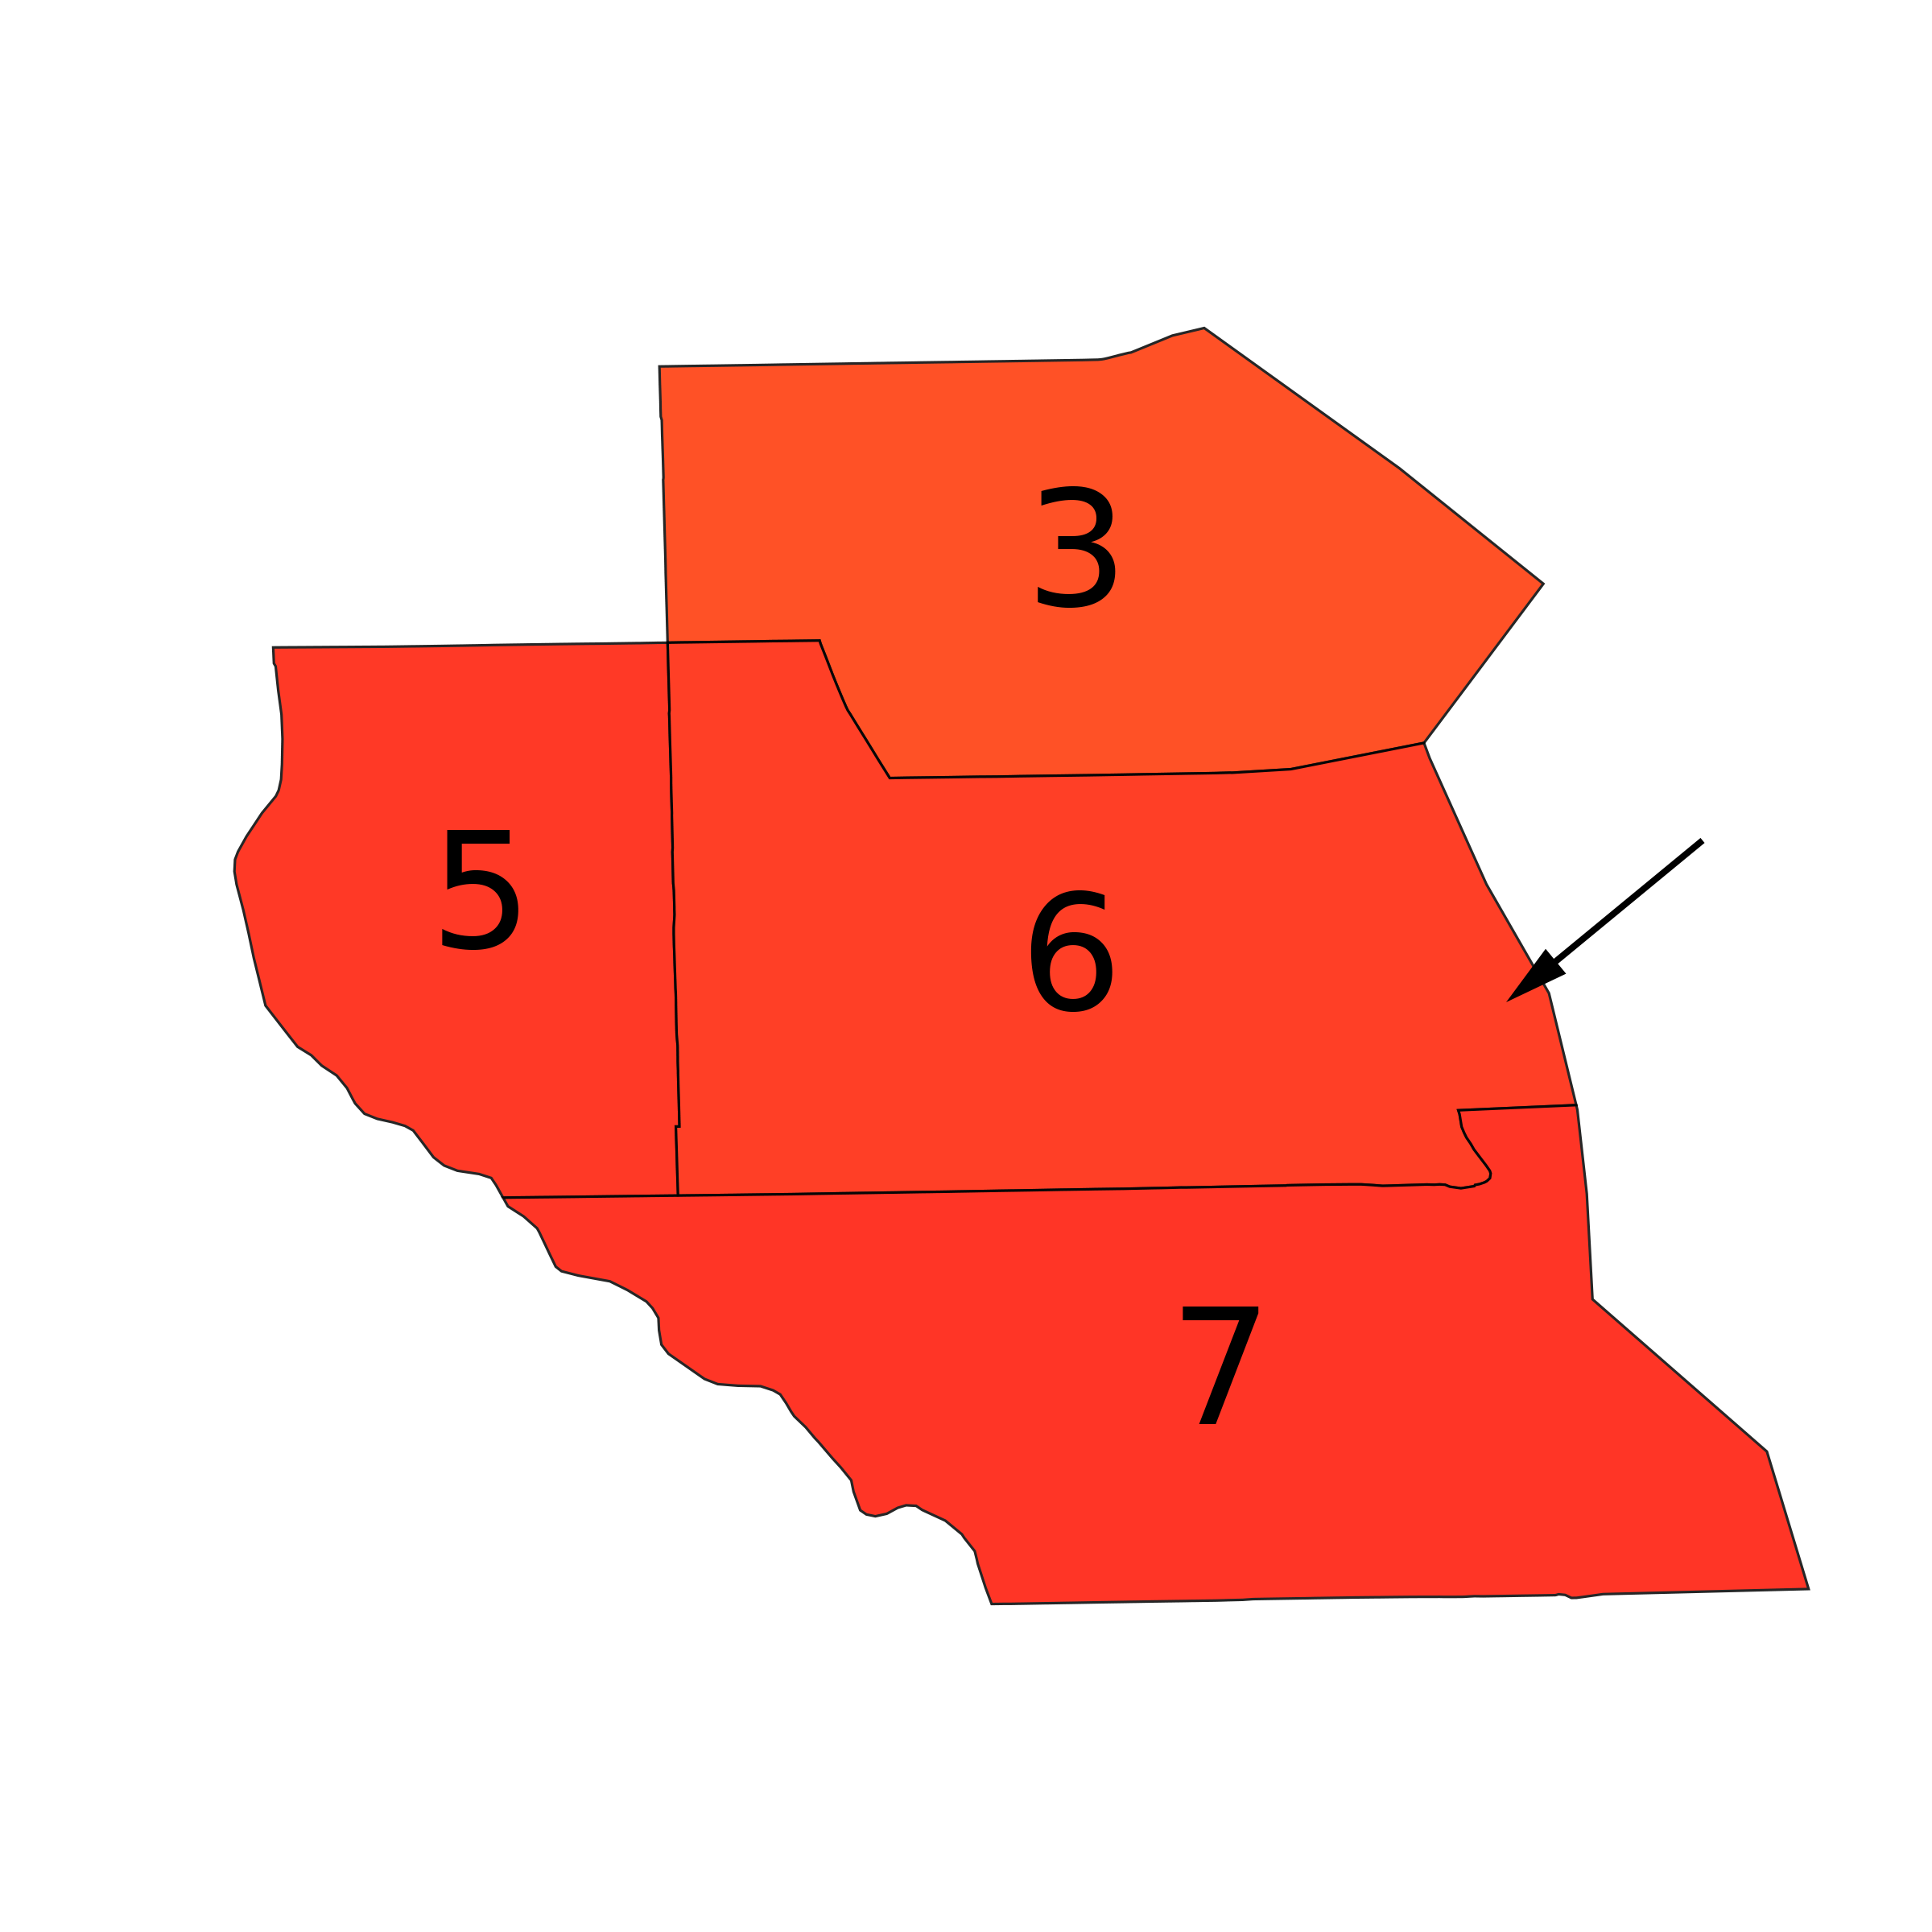
\includegraphics[width=0.2\linewidth]{fig/before-train_average_house_price.png}}
\subfigure[After]{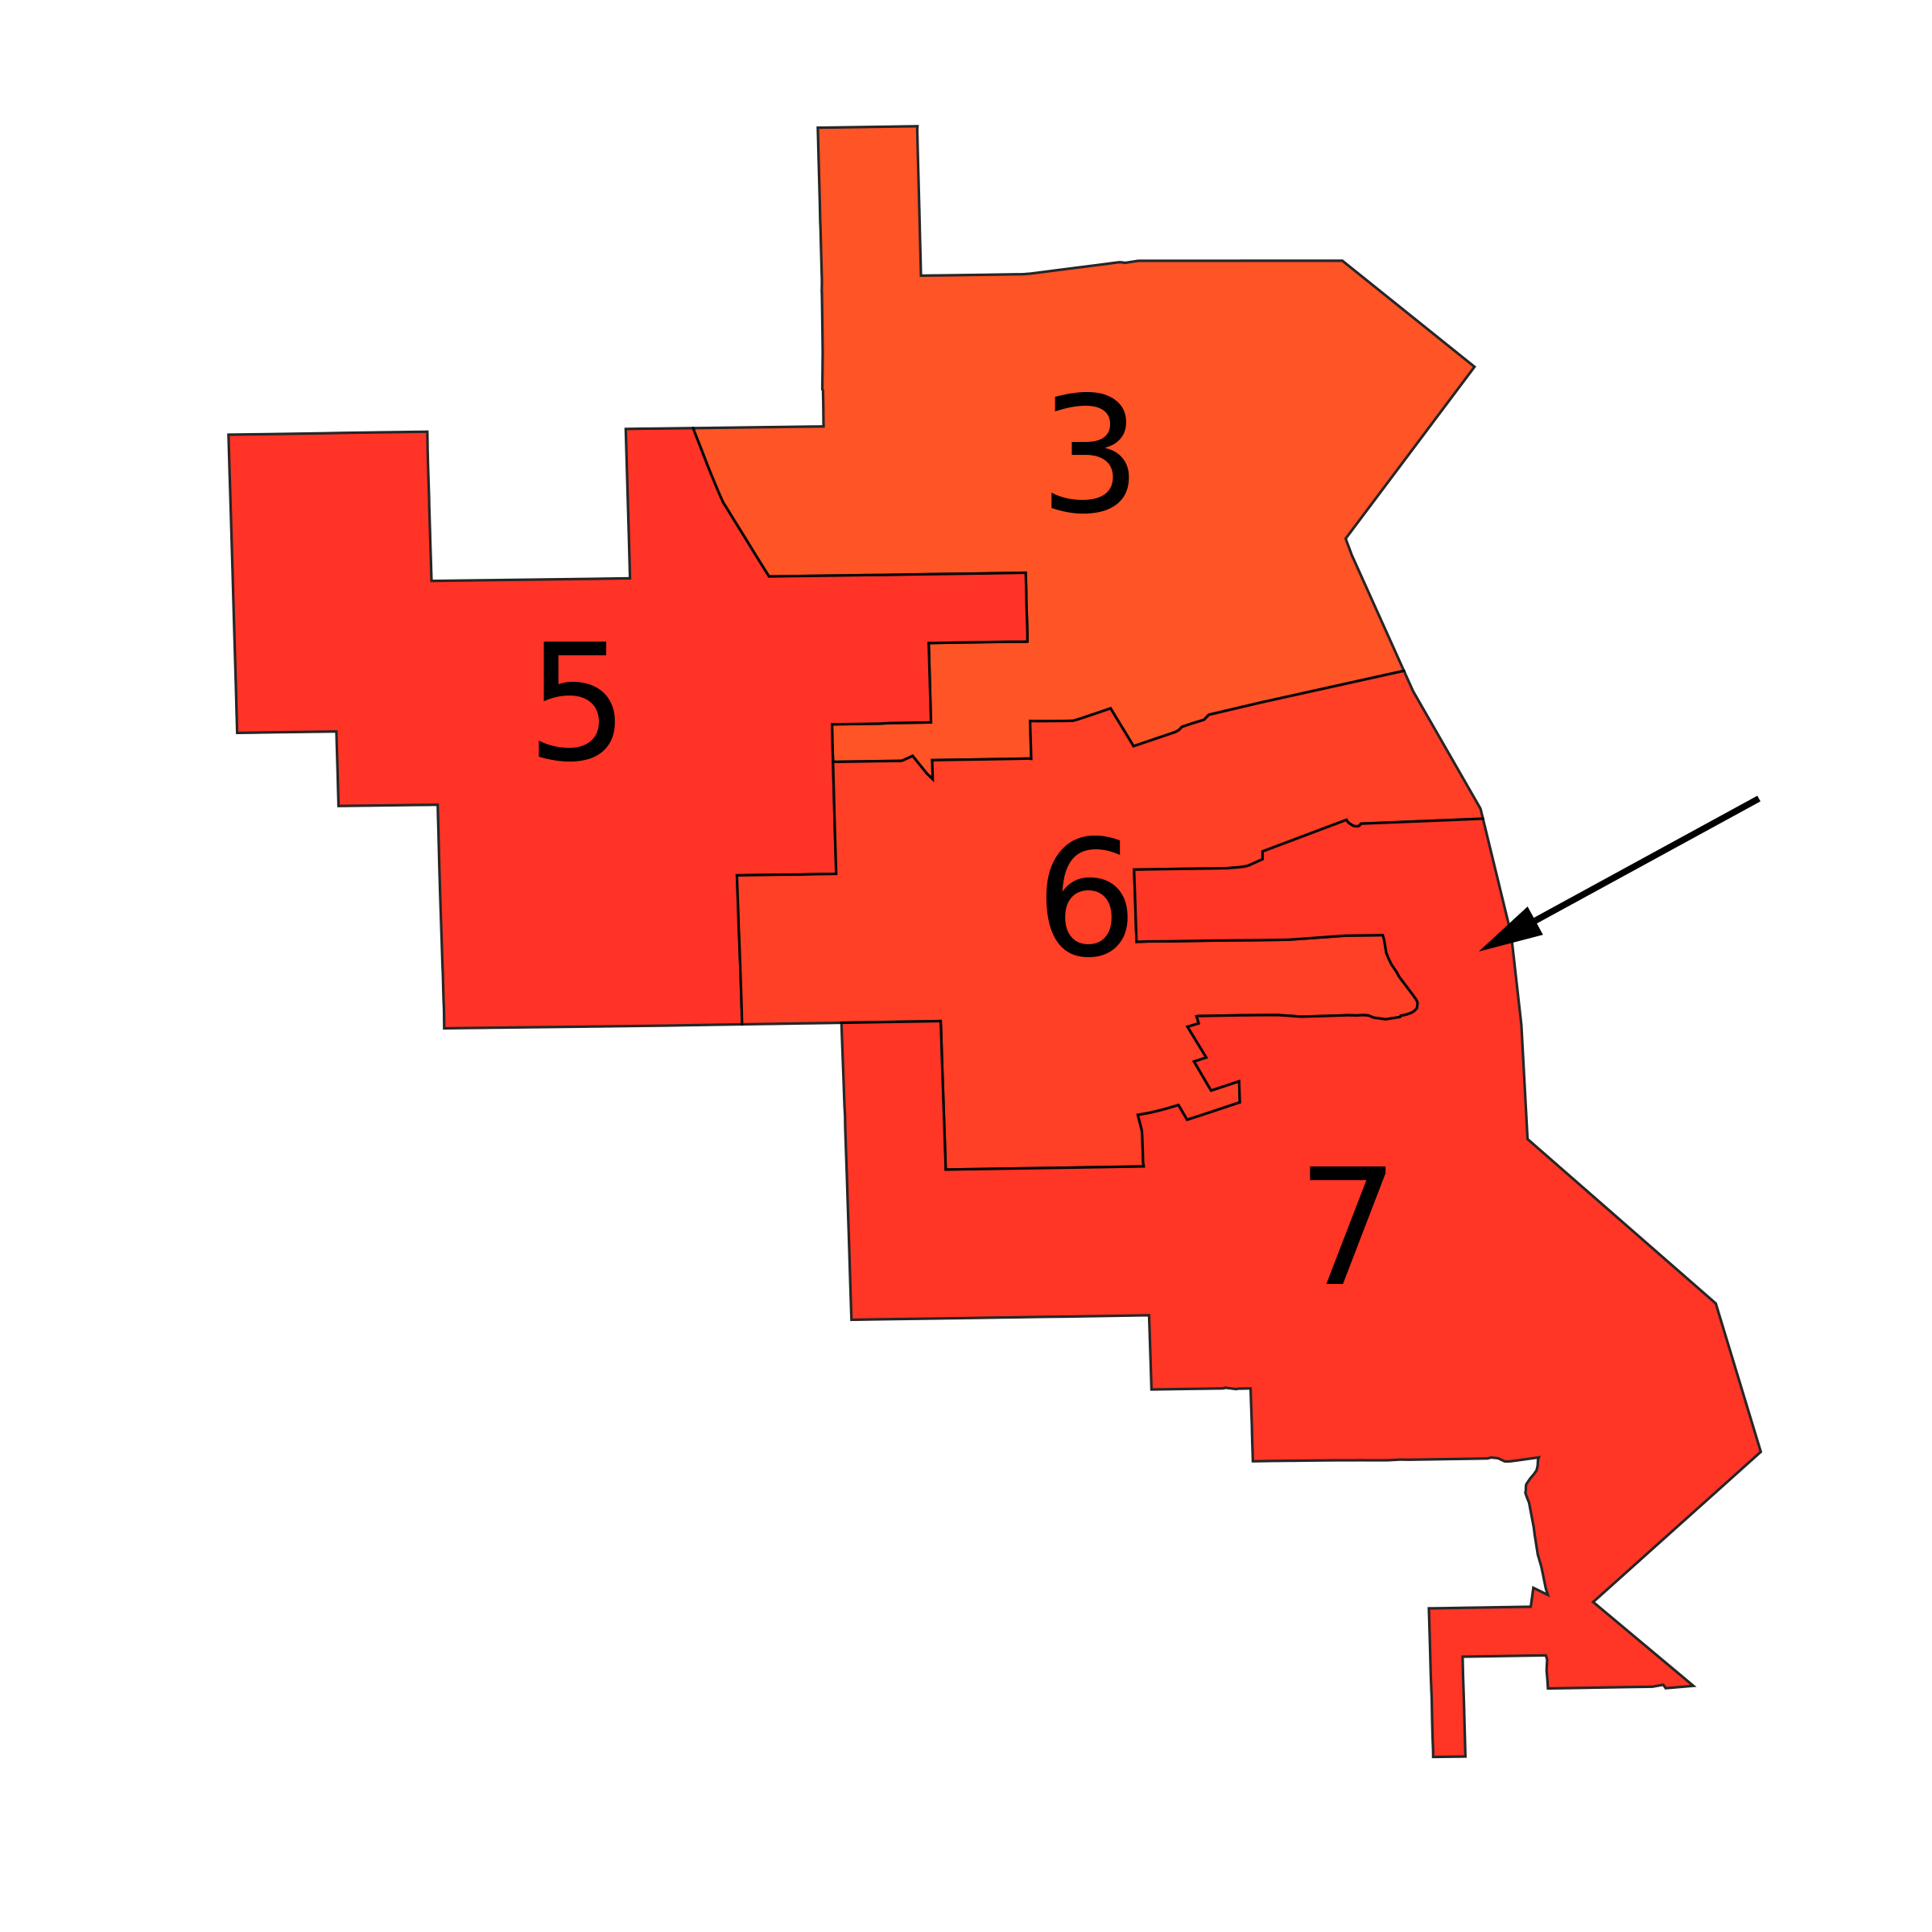
\includegraphics[width=0.2\linewidth]{fig/after-train_average_house_price.png}}
\subfigure[Lake View]{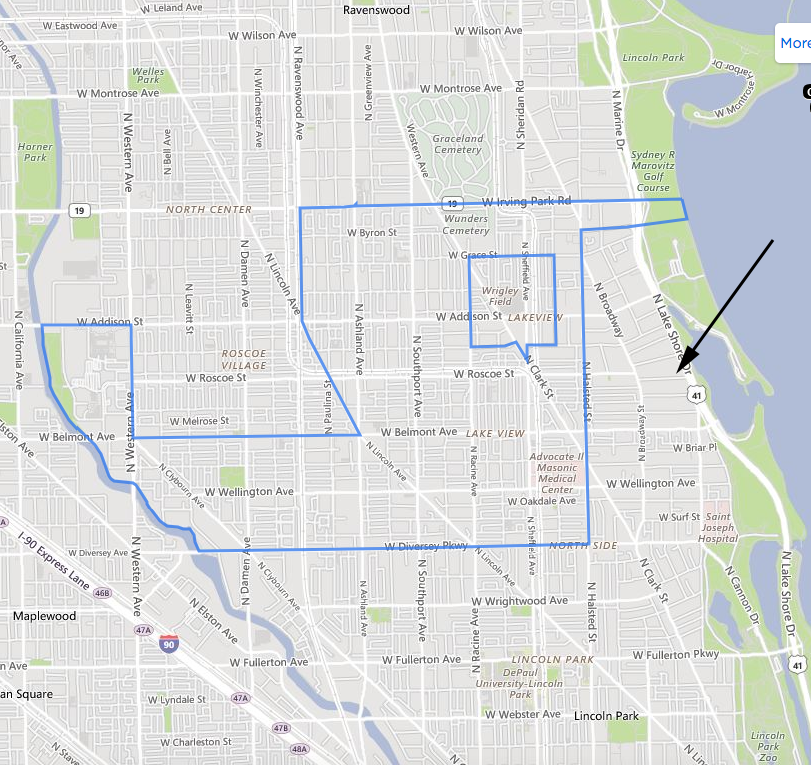
\includegraphics[width=0.2\linewidth]{fig/ca-lakeview.png}}
\subfigure[Lake View East]{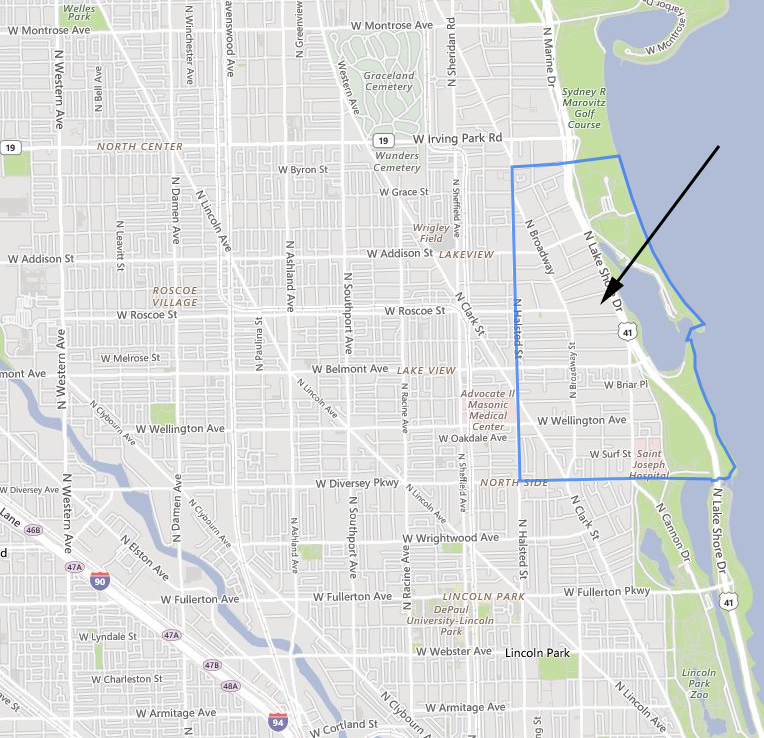
\includegraphics[width=0.2\linewidth]{fig/ca-lakeview-east.png}}
\caption{Average house price (per square foot) by community area. (a) All communities in the city of Chicago. Arrow denotes region of interest. (b) Region of interest, viewed with administrative boundaries. Arrow denotes coastal area near Belmont Harbor. (c) Region of interest viewed with optimal partition from Q-learning. Arrow denotes coastal area near Belmont Harbor. (d) Region of interest according to Zillow, Lake View area. Arrow denotes coastal area near Belmont Harbor, which falls outside of Lake View. (e) The Belmont Harbor area is split into a separate community, Lake View East}
\label{fig:housePrice}
\end{figure*}

We focus our discussion on the house price prediction task. First, we visualize a heat map of house price (per square foot) for the whole city of Chicago, found in figure \ref{fig:housePrice}a. Warmer colors (red) denote greater prices, while cooler colors (yellow) indicate lower prices. The arrows in the figure point to the region of interest for our discussion, near community \#6. This is the same outlier community in the crime prediction task. Notice that all three of the adjacent communities all have similar colors, which in turn means they have similar average house price values. The original community partition \#6 (called the Lake View area) stretches east and west, and encompasses the entire coastal area between community \#3 and \#7. See figure \ref{fig:housePrice}b for a visualization. However, the region of interest indicated by the arrow is semantically very different from census tracts farther west and closer community \#5. The coastal region of interest contains Belmont Harbor, one of Chicago's largest boating areas. Notice that the the Q-learning method divides community area \#6 and groups the coastal tracts surrounding the Belmont Harbor with other coastal areas farther south. This natural division is apparent from figure \ref{fig:housePrice}c. These additional regions contain other leisure destinations such as the Lincoln Park Zoo, and numerous beach areas. This semantic argument is bolstered by an independent source: Zillow's own self-defined regions. Figure \ref{fig:housePrice}d shows the same region of interest, community area \#6 on Zillow.com. Zillow breaks the original community \#6 into Lake View (figure \ref{fig:housePrice}d) and Lake View East (figure \ref{fig:housePrice}e). The region partition chosen by Q-learning is similar to Zillow's self-defined region in that they both exclude the coastal, Belmont Harbor area from the original community \#6 (Lake View neighborhood). While the two regions are not exactly the same, it is interesting to note that they both removed the Belmont Harbor area from the original community.

The proposed partition from Q-learning (figure \ref{fig:housePrice}c) is superior to the original community partition when used in conjunction with a predictive, statistical model. Note that this partition could not have been achieved by simply using the house price feature alone in any clustering algorithm. The reasons for this are twofold. First, the four community regions in figure \ref{fig:housePrice}b have nearly identical colors, and in turn, nearly identical average house prices. It is unlikely a canonical clustering algorithm would be able to discover any meaningful divisions between the underlying tracts using house price alone. Second, the performance of the agglomerative clustering algorithm in section \ref{benchmarks} is extremely poor. If simple clustering were effective, this algorithm would likely have discovered the proper pattern. In contrast, the Q-learning algorithm learns the spatial correlation between the features and house prices, rather than the similarities in house price alone. By discovering the underlying joint distribution of the features and house price, the algorithm is able to learn partitions that are more meaningful. 





